\documentclass[12pt]{article}

\usepackage{amsmath}
\usepackage{mathtools}
\usepackage{amsfonts}
\usepackage{graphicx}
\usepackage{bbm}
\usepackage{mathptmx}
\usepackage[margin=1in]{geometry}
\setlength{\parindent}{0in}

\title{Probability Theory}
\author{Oualid Merzouga}

\begin{document}

\maketitle
\pagenumbering{gobble}
\newpage
\pagenumbering{arabic}



\section{Set Theory}
\begin{align*}
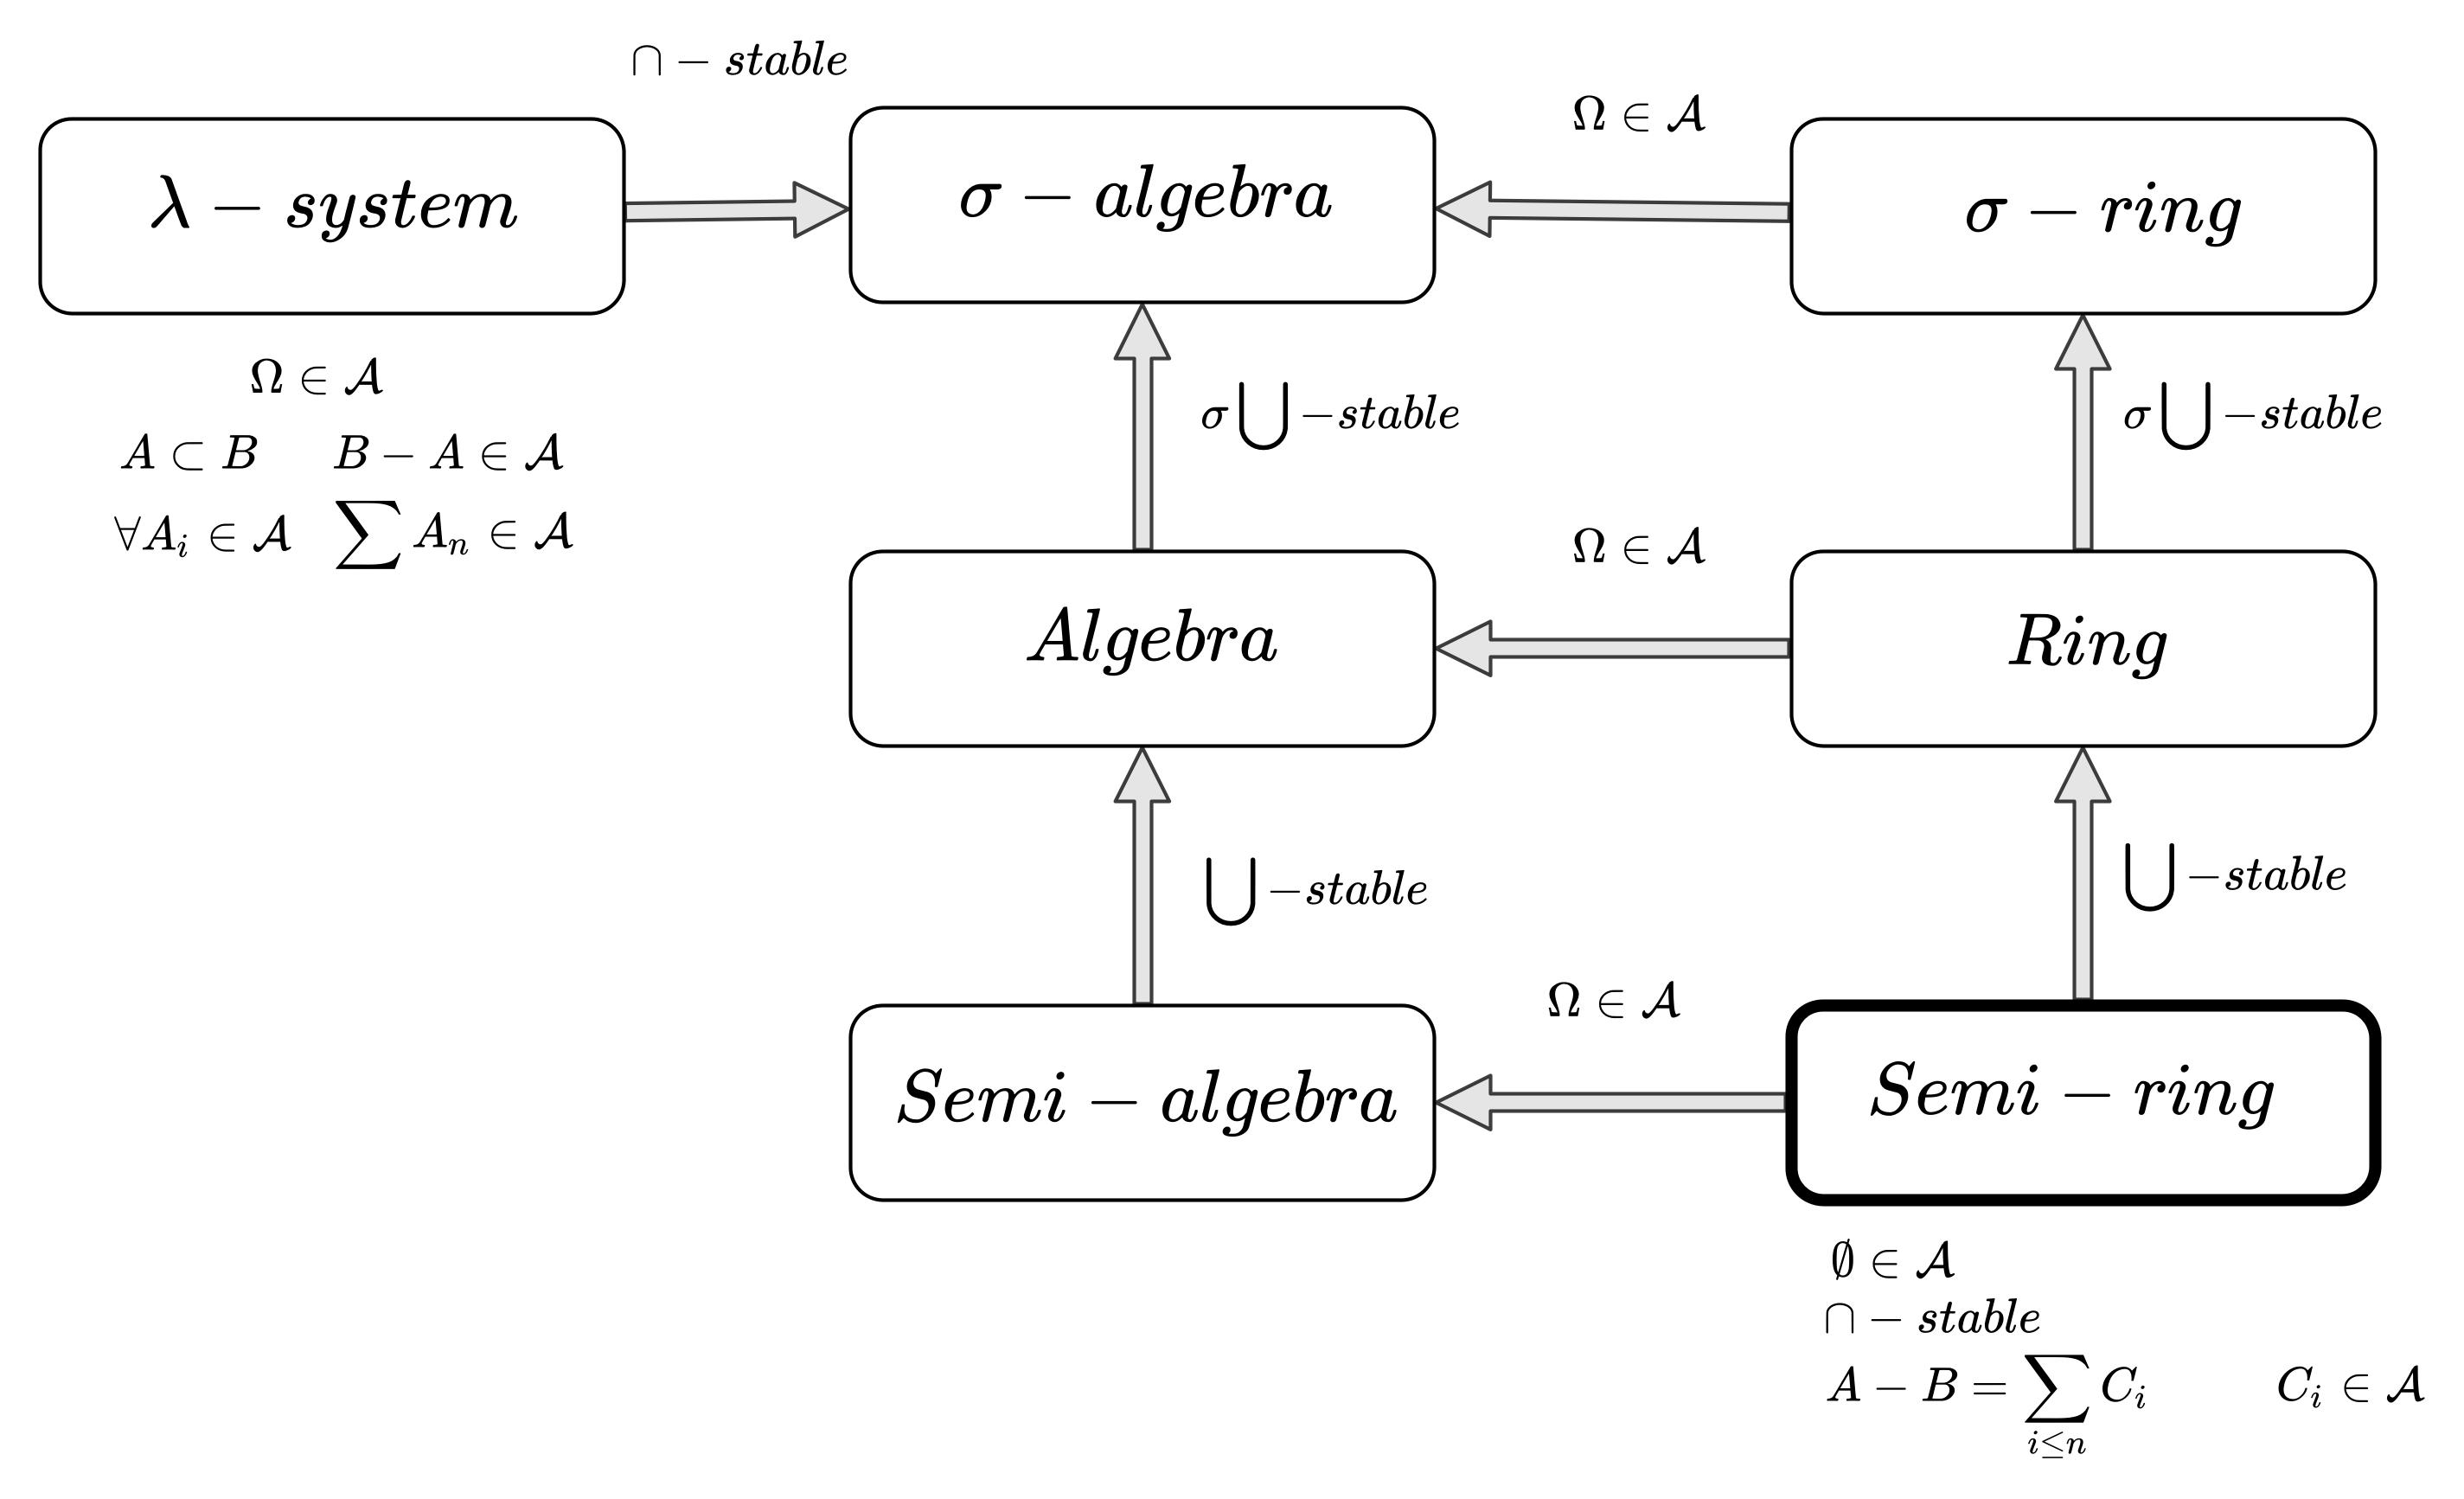
\includegraphics[scale=0.5]{../images/Sets2.png}
\end{align*}


\section{Measures}

\subsection{Definitions}

$(X,S)$ is a $\textbf{measurable space}$ if $S$ is a sigma algebra and $\bigcup S = X$

$(X,S,\mu)$ is a $\textbf{measure space}$ if $(X,S)$ is a measurable space and $\mu$ a measure defined on $S$

$E$ is a $\textbf{measurable set}$ if $E\in S$.

$\mu : \xi \rightarrow \mathbb{R}$ s.t $\xi$ is a class of sets of $X$ is a $\textbf{set function}$

A set function $\mu : \xi \rightarrow [0, \infty]$ defined on a semi-ring $\xi$ is :

\begin{itemize}
\item $\textbf{Content}$ if additive
\item A $\textbf{premeasure}$ if countably additive
\item A $\textbf{measure}$ if is a premeasure on a $\sigma$-algebra
\item A $\textbf{probability measure}$ if is a measure with $\mu(\Omega) = 1$
\end{itemize}

$A$ and $B$ respectively positive and negative  with respect to $\mu$ are a $\textbf{Hahn decomposition}$ of $X$ if $X = A \cup B$ and $A \cap B = \emptyset$ 

\subsection{Properties of set functions}
\begin{itemize}

\item Finitly additive: 
 $E_1 \dots E_n \in \xi \implies \mu(\sum_{i=1}^n E_i) = \sum_{i=1}^n \mu(E_i)$
 
\item Countably additive: 
 $E_1 \dots \in \xi \implies \mu(\sum_{i=1}^{\infty} E_i) = \sum_{i=1}^{\infty} \mu(E_i) $

\item Finite: 
 $E \in \xi \implies \left |\mu(E) \right| < \infty $

 \item Continuous from below
\[ \left.
\begin{array}{l l}
\star \; E \in \xi \\
\star \; \forall i \; E_i \in \xi \\
\star \; (E_n)_{n \in \mathbb{N}} \uparrow E \\
\end{array}
\right\} \lim_{n \to\infty}\mu(E_n) = \mu(E) \]

\item Continuous from above
\[ \left.
\begin{array}{l l}
\star \; E \in \xi \\
\star \; \forall i \; E_i \in \xi \\
\star \; (E_n)_{n \in \mathbb{N}} \downarrow E \\
\star \; \exists m$ s.t $|\mu(E_m)| < \infty 
\end{array}
\right\} \lim_{n \to\infty}\mu(E_n) = \mu(E) \]

\end{itemize}



\newpage
\section{\LARGE Measurable functions and transformations}

\subsection{Definitions}
Let $(X,S)$ and $(Y,G)$ be measurables spaces space

$T : X \rightarrow Y$ is a $\textbf{measurable transformation}$ if for $B\in G$: 
\begin{align}
T^{-1}(G) \in S
\end{align}

In particular $f:D \rightarrow \mathbb{R}$ is a $\textbf{measurable function}$ if :
\begin{align}
D &\in S\\
\{x &\in D:f(x) \leq a\} \in S 
\end{align}

$f_+$ is the $\textbf{positive part}$ of $f$ if:

\begin{align}
f_+(x) = 
\begin{cases}
f(x) \;&if \;f(x) > 0\\ 
0 \;&if \;f(x) \leq 0
\end{cases}
\end{align}

$f_-$ is the $\textbf{negative part}$ of $f$ if:

\begin{align}
f_-(x) = 
\begin{cases}
-f(x) \;&if \;f(x) < 0\\ 
0 \;&if \;f(x) \geq 0
\end{cases}
\end{align}



$\mathbbm{1}_E : X \rightarrow \{0,1\}$ is a $\textbf{characteristic function}$ or $\textbf{indicator function}$ on the subset $E \subset X$ if :

\begin{align}
\mathbbm{1}_E(x) = 
\begin{cases}
1 \;if \;x \in E\\ 
0 \;if \;x \notin E
\end{cases}
\end{align}

$f : X \rightarrow \mathbb{R}$ is a $\textbf{simple function}$ if for $a_i \in \mathbb{R}$ and $E_i \in S$ disjoints we have :

\begin{align} f(x) = \sum_{i=1}^na_i\mathbbm{1}_{E_i}(x)\end{align}

\subsection{Properties of measurable functions}
\begin{itemize}
\item If $(f_i)_{i\in\mathbb({N}}$ measurable functions with $a_i \in \mathbb{R}$ then : $\sum_i a_if_i$, $fg$, $f/g$  are measurable
\item If $f,g$ measurable functions $\rightarrow$ $\{f(x) = g(x)\}$ $\{f(x) \leq g(x)\}$ $\{f(x) < g(x)\}$ are measurable sets
\item If $f$ is measurable then $|f(x)|^a$ is measurable $\forall a \in \mathbb{R}$
\item If $\{f_n\}$ a sequence of measurable functions, then $\lim_{i \rightarrow \infty}f_n(x) = f(x)$ is measurable
\item If $T:X \rightarrow Y$ measurable transformation, then $\mu(T^{-1})$ is a measure on $G$
\end{itemize}

\newpage
\section{Integration}

\subsection{Definitions}
$L_1$ is the class of integrable functions

A non negative, measurable function $f$ is $\textbf{integrable}$ if $\int f < \infty$

A measurable function $f$ is $\textbf{integrable}$ if $f_+$ and $f_-$ are integrables 

\subsection{Integration of functions}
\begin{itemize}
\item Integral of characteristic function
Let $(X,S,\mu)$ be a measure space and $E\in S$

\begin{align}
\int \mathbb{1}_E d\mu =  \mu(E)
\end{align}


\item Integral of non negative, simple function

Let $(X,S,\mu)$ be a measure space, $E_1 \dots E_n$, disjoints sets of $S$ where $\bigcup E_i = X$ and $f = \sum_{i=1}^na_i\mathbb{1}_{E_i}$

\begin{align}
\int fd\mu =  \sum_{i=1}^na_i\mu(E_i)
\end{align}

Note : For simple functions $\int$ and $\lim$ commute


\item Integral of non negative, measurable function

Let $(X,S,\mu)$ be a measure space,  $f$ non negative measurable function, $(f_n)_{n \in \mathbb{N}} \uparrow f$ s.t $\forall i \;f_i$ simple functions with $\lim_{n \to \infty}f_n(x) = f(x)$ 

\begin{align}
\int fd\mu =  \lim_{n \to \infty}\int f_nd\mu
\end{align}

Note : $\mu(E) = 0 \implies \int_E fd\mu = 0$ with $E \in S$
    

\item Integral of non negative, measurable function a.e

Let $(X,S,\mu)$ be a measure space, $f$ non negative, measurable function a.e, $g$ non negative, measurable function with $f = g$ a.e

\begin{align}
\int fd\mu =  \int gd\mu
\end{align}


\item Integral of measurable function a.e

Let $(X,S,\mu)$ be a measure space, $f$ measurable function a.e, $f_+$ and  $f_-$ non negative, measurable functions a.e whith $f = f_+ - f_-$

\begin{align}
\int f =  \int f_+ - \int f_-
\end{align}
\end{itemize}

\subsection{Properties of the integral}
\begin{itemize}

\item $f$ integrable $\implies$ $f$ finite a.e

\item $(f_i)_{i\in \mathbb{N}}$ are integrable functions then :
\begin{align}
\int \sum_{i\in \mathbb{N}} f_id\mu = \sum_{i\in \mathbb{N}} \int f_id\mu
\end{align}

\item $f \in L_1 \iff f_+, f_- \in L_1 \iff |f| \in L_1$
\end{itemize}


\subsection{Theorems}
\begin{itemize}
\item Monotone Convergence Theorem \\

Let $(X,S,\mu)$ be a measure space, $(f_n)_{n \in \mathbb{N}}$ monotone increasing sequence of non negative, measurable, functions a.e, $f$ non negative, measurable function with $ \lim_{n \to \infty}f_n(x) = f(x)$, $x\in X$ a.e

\begin{align}
\lim_{n \to \infty}\int f_nd\mu = \int fd\mu
\end{align}

\item Fatou's Lemma \\
Let $(X,S,\mu)$ be a measure space, $(f_n)_{n \in \mathbb{N}}$ monotone increasing sequence of non negative, measurable, functions a.e

\begin{align}
\lim_{n \to \infty}\inf\int f_nd\mu = \int(\lim_{n \to \infty}\inf f_n)d\mu
\end{align}

\item Dominated convergence \\
Let $(X,S,\mu)$ measure space, $(f_n)_{n \in \mathbb{N}}$ sequence of integrable functions, $g$ integrable function s.t $\forall n$, $\left|f_n\right| \leq \left|g\right|$ a.e, f measurable function s.t $f_n(x) \rightarrow f(x)$ a.e

\begin{align}
f &\in L_1 \\ 
\int \left|f_n - f\right|d\mu &\rightarrow 0
\end{align}


\item Transformation theorem  \\
Let $(X,S,\mu)$ measure space, $(Y,\xi)$ measurable space, $T : X \rightarrow Y$ Transformation defined a.e, $f : Y \rightarrow \mathbb{R}$ measurable function

\begin{align}
\int_Y fd(\mu T^{-1}) = \int_X fTd\mu
\end{align}

\item Radon-Nikodym theorem  \\
Let $(X,S,\mu)$ totally $\sigma$-finite measure space, $ v << \mu $ with $v$ $\sigma$-finite signed measure on $S$

\begin{align}
&\exists f:X\rightarrow [0,\infty)\text{measurable} \\
&v(E) = \int fd\mu\;\;\; \forall E\in S
\end{align}

Notationwise: $f = \cfrac{dv}{d\mu}$

\item Lebesgue decomposition

Let $(X,S)$ be a measurable space, $\mu$ and $v$ $\sigma$ -finite signed measure on $S$

\begin{align}
\exists v_1, v_2 \;\; s.t \;\; v &= v_1 + v_2 \\
v_0 &\perp \mu \\
v_1 &<< \mu
\end{align}

\item Generated measures

Let $(X,S,\mu)$ be a measure space, $g:X\rightarrow [0,\infty]$ measurable, $v(E) = \int_E gd\mu$


\begin{align}
\text{Then $v$ is a measure on $(X, S)$ and for any $f:X\rightarrow \mathbb{R}$}
\int_X fdv = \int_X fgd\mu
\end{align}

\end{itemize}


\newpage
\section{Product spaces}
\subsection{Definitions}
Let $(X,\mathcal{S},\mu)$ and $(W,\mathcal{W})$ be respectively a measure space and a measurable space.

$X\times W = \{(x,y) : x \in X, y \in W\}$ is called the $\textbf{product space}$.

$T_x:(X\times W ) \longmapsto  X$ is called the $\textbf{X-section}$ or the $\textbf{Projection function}$ if $T_x(x,w) = x$
\subsection{Mixture of measures}
Let $v : (X, \mathcal{W}) \longmapsto \mathbb{R} $ be a function defined by :
\begin{align*}
&v(\bullet, E) = v_x(E) \text{ measure on $\mathcal{W}$ for $x \in X$ fixed} \\
&v(x, \bullet) = v_E(x) \text{ is $\mathcal{S}$-measurable for $E \in \mathcal{W}$ fixed} \\
&\text{f is always assumed to be measurable non negative}
\end{align*}

\begin{itemize}
\item $\underline{\text{Integration of }f:W \longmapsto \mathbb{R} \quad w.r.t \quad \lambda \:on\: \mathcal{W}}$

For $E \in \mathcal{W}$ we define the measure :
\begin{align*}
\lambda(E) = \int_X v_E(x)\:d\mu(x)\quad \text{is a measure on } \mathcal{W}
\end{align*}
Let's define the non negative $\mathcal{S}$-measurable function a.e as :

\begin{align*}
g : X &\longmapsto \mathbb{R} \\
x &\longmapsto \int_{\mathcal{W}}f(E)\:dv_x(E) = \int f\:dv_x
\end{align*}
We have then : 

\begin{align*}
\int_{\mathcal{W}}f(E)\:d\lambda(E) &= \int_X\Big(\int_{\mathcal{W}}f(E)\:dv_x(E)\Big)d\mu(x) \\
\int_{\mathcal{W}}f\:d\lambda &= \int_X\int_{\mathcal{W}}f\:dv_xd\mu
\end{align*}
\end{itemize}

\subsection{Product measure}
For $E = A \times B$ we take the measure $v$ to be non dependent on x. So the product measure becomes :

\begin{align}
\lambda(E) &= \int_X v_B\mathbbm{1}_A\:d\mu(x) \\
\lambda(E) &= v(B)\mu(A)
\end{align}

\subsection{Fubini's Theorem}
\begin{itemize}
\item $(X, \mathcal{S}, \mu)$ and $(Y, \mathcal{T}, \mathcal{v})$ $\sigma$-finite measure spaces

\item f is an $\mathcal{S} \times \mathcal{T}$-measurable non negative function defined a.e $(\lambda = \mu \times \mathcal{v})$

\begin{align}
\int_{X \times Y}fd\lambda = \int_X \Big(\int_Yf_xd\mathcal{v}\Big)d\mu(x) = \int_Y \Big(\int_Xf_yd\mu\Big)d\mathcal{v}(y)
\end{align}

\end{itemize}


\newpage

\section*{\LARGE Random Elements}

\subsection*{Definitions}

$(\Omega, \mathcal{F}, P)$ is a $\textbf{Probability space}$

\noindent A $\textbf{Random variable}$ is a measurable function $X : \Omega \rightarrow \mathbb{R}$

\noindent A $\textbf{Random element}$ is a measurable transformation $X : \Omega \rightarrow Y$ with $(Y, \mathcal{S})$ measurable space.

\noindent The $\textbf{Distribution}$ of X is the induced measure:

\begin{align*}
P_X : \sigma(Y) &\longmapsto [0,1] \\
    B &\longmapsto P\{\omega: X(\omega) \in B\} \quad &\text{(written also $P\{X \in B\}$)} \\
B &\longmapsto P\{\omega \in X^{-1}(B)\} &\text{(written also $PX^{-1}(B)$)}
\end{align*}

\noindent The $\textbf{Distribution function}$ of X is defined as: 

\begin{align*}
    F:\mathbb{R} &\longmapsto \mathbb{R} \\
x &\longmapsto P_X(-\infty, x)
\end{align*}

\noindent The $\textbf{Expectation}$ of a random variable $X$ is $E(X) = \displaystyle\int_{\Omega} X(\omega)dP(\omega)$


\subsection*{Sum of two Random variables}
Let $X,Y$ be two random variables. Let $\phi(x_1,x_2) = x_1 + x_2$. We have the distribution:

\begin{align*}
P\{\omega: X(\omega)+Y(\omega) \in B\} &= P\{X+Y \in B\} \\
&= P\{\phi(X,Y) \in B\} \\
&= P\{(X,Y) \in \phi^{-1}B\} \\
&= \int \mathbbm{1}_{\phi^{-1}B}(x,y)\;dP(X^{-1}\times Y^{-1}) \\
&= \iint \mathbbm{1}_{\phi^{-1}B}(x,y)\;dPX^{-1}\; dPY^{-1} \\
&= \int PX^{-1}(B-y) dPY^{-1} = \int PY^{-1}(B-x) dPX^{-1} \\
&= \int P_X(B-y) dP_Y = \int P_Y(B-x) dP_X \\
&= \int_{-\infty}^{\infty} P_X(B-y) dP_Y(y) = \int_{-\infty}^{\infty} P_Y(B-x) dP_X(x) \\
\end{align*}

We derive the distribution function:

\begin{align*}
P\{X+Y < z\} = F_{X+Y}(z) &= \int_{-\infty}^{\infty} P_Y((-\infty, z] - x) dP_X(x) = \int_{-\infty}^{\infty} P_X((-\infty, z] - y) dP_Y(y) \\
&= \int_{-\infty}^{\infty} F_Y(z - x) dP_X(x) = \int_{-\infty}^{\infty} F_X(z - y) dP_Y(y)
\end{align*}


\subsection*{Discrete random variable}

$P_X$ is called $\textbf{discrete}$ if it  takes values in a countable set $\mathcal{C} = \{c_1,c_2,\dots\}$ s.t $P_x(\mathcal{C}^c) = 0$

We have the random variable: 

\begin{align*}
X : \Omega &\longmapsto \mathcal{C} \\
\omega &\longmapsto c_i
\end{align*}

\begin{itemize}
\item Distribution

We derive the distribution : 

\begin{align*}
P_X : \sigma(\mathcal{C}) &\longmapsto [0,1] \\
B &\longmapsto P\{X^{-1}(B)\} = P\Big\{X^{-1}\Big(\bigcup_{c_i \in B} c_i\Big)\Big\} = P\Big\{\bigcup_{c_i \in B}X^{-1}(\{c_i\})\Big\} \\
B &\longmapsto \boxed{\displaystyle\sum_{c_i \in B} PX^{-1}(\{c_i\})} \quad \Big( = \sum_{c_i \in B} p_X(c_i) = \sum_{c_i \in \mathcal{C}} p_X(c_i) \mathbbm{1}_B(c_i)\Big)
\end{align*}

\item Probability mass function

$p_X$ (Distribution restricted to sample space) is called the $\textbf{probability mass function}$ defined by :

\begin{align*}
p_X:\mathcal{C} &\longmapsto [0,1] \\
c_i &\longmapsto P_X(c_i)
\end{align*}


\item Expectation

When $\mathcal{C} \subset \mathbb{R}$ we have for $I$ countable index set : $\mathcal{C} = \bigsqcup_i \{c_i\}$. We have then :

\begin{align*}
    X(\omega) &= \sum_{c_i \in \mathcal{C}} c_i\mathbbm{1}_{X^{-1}\{c_i\}}(\omega) \\
E(X) &= \int_{\Omega} \sum_{c_i \in \mathcal{C}} c_i\mathbbm{1}_{X^{-1}\{c_i\}}(\omega) dP(\omega) \\ 
&= \sum_{c_i \in \mathcal{C}} c_iP(X^{-1}\{c_i\}) \\ 
E(X) &= \boxed{\displaystyle\sum_{c_i \in \mathcal{C}} c_ip_X(c_i)} \\
\end{align*}


\item Sum of two discrete random variables

Let $\mathcal{C}_1, \mathcal{C}_2$ be coutable sets and $X_i:\Omega \longmapsto \mathcal{C}_i \quad i \in \{1,2\}$ be random variables. 


\begin{align*}
P\{X_1+X_2 \in B\} &= \int_{\mathbb{R}} P_{X_1}(B-x_2) dP_{X_2}(x_2) \quad &\text{Definition }\\
&=\int_{\mathbb{R}} \sum_{c_i \in \mathcal{C}_1} p_{X_1}(c_i)\mathbbm{1}_{\{B-x_2\}}(c_i) dP_{X_2}(x_2) &\text{Expanding $P_{X_1}$} \\
&=\int_{\mathbb{R}} \sum_{c_i \in \mathcal{C}_1} p_{X_1}(c_i)\mathbbm{1}_{\{B-c_i\}}(x_2) dP_{X_2}(x_2) &\text{$c_i \in B-x_2 \implies x_2 \in B-c_i$}\\
&=\sum_{c_i \in \mathcal{C}_1} p_{X_1}(c_i)P_{X_2}(B-c_i) \\
&=\sum_{c_i \in \mathcal{C}_1}\sum_{b_i \in \mathcal{C}_2} p_{X_1}(c_i) p_{X_2}(b_i)\mathbbm{1}_{\{B-c_i\}}(b_i) \\
&=\boxed{\displaystyle\sum_{c_i \in \mathcal{C}_1}\sum_{b_i \in \{B - c_i\}}p_{X_1}(c_i) p_{X_2}(b_i)}
\end{align*}


\end{itemize}


\subsection*{Continuous random variable}
$P_X$ absolutly continuous w.r.t the Lebesgue measure $\mu$:

\begin{align}
P_X << \mu &\implies \exists \; p_d \quad s.t \quad P_X = \int p_d(x)d\mu
\end{align}
The function $p_d$ is then called the $\textbf{Probability density function}$



\newpage
\subsection*{Conditional Expectation and probabilities}
Let $\mathcal{G} \subseteq \mathcal{F}$ be a sub $\sigma$-algebra and $X:\Omega \longmapsto \mathbb{R}$ a measurable function. Let $P_{|\mathcal{G}}$ be the restriction of $P$ on $\mathcal{G}$. We have : $P_{|\mathcal{G}} = P/P(\mathcal{G})$ and then :

\begin{align*}
    P(X\in A | B)   &= \int_B \mathbbm{1}_{X^{-1}A}dP_B \\
		    &= \frac{1}{P(B)}\int_B \mathbbm{1}_{X^{-1}A}dP \\
		    &= \frac{1}{P(B)} P(X\in A \cap B)
\end{align*}

\begin{align*}
    \mathbb{E}(X | B)	&= \int_B XdP_B \\
			&= \int_B Xd(P/P(B)) \\
			&= \frac{1}{P(B)} \int_B XdP 
\end{align*}




\end{document}
